\hypertarget{_shape_8hpp}{
\subsection{Shape.hpp File Reference}
\label{_shape_8hpp}\index{Shape.hpp(171)@{Shape.hpp(171)}}
}
Declaration of \hyperlink{class_shape}{Shape} class.  


{\tt \#include $<$vector$>$}\par
{\tt \#include $<$utility$>$}\par


Include dependency graph for Shape.hpp:\nopagebreak
\begin{figure}[H]
\begin{center}
\leavevmode
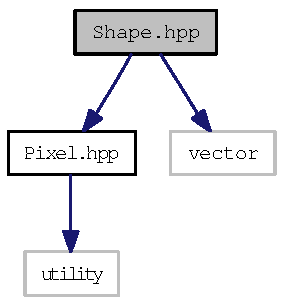
\includegraphics[width=78pt]{_shape_8hpp__incl}
\end{center}
\end{figure}


This graph shows which files directly or indirectly include this file:\nopagebreak
\begin{figure}[H]
\begin{center}
\leavevmode
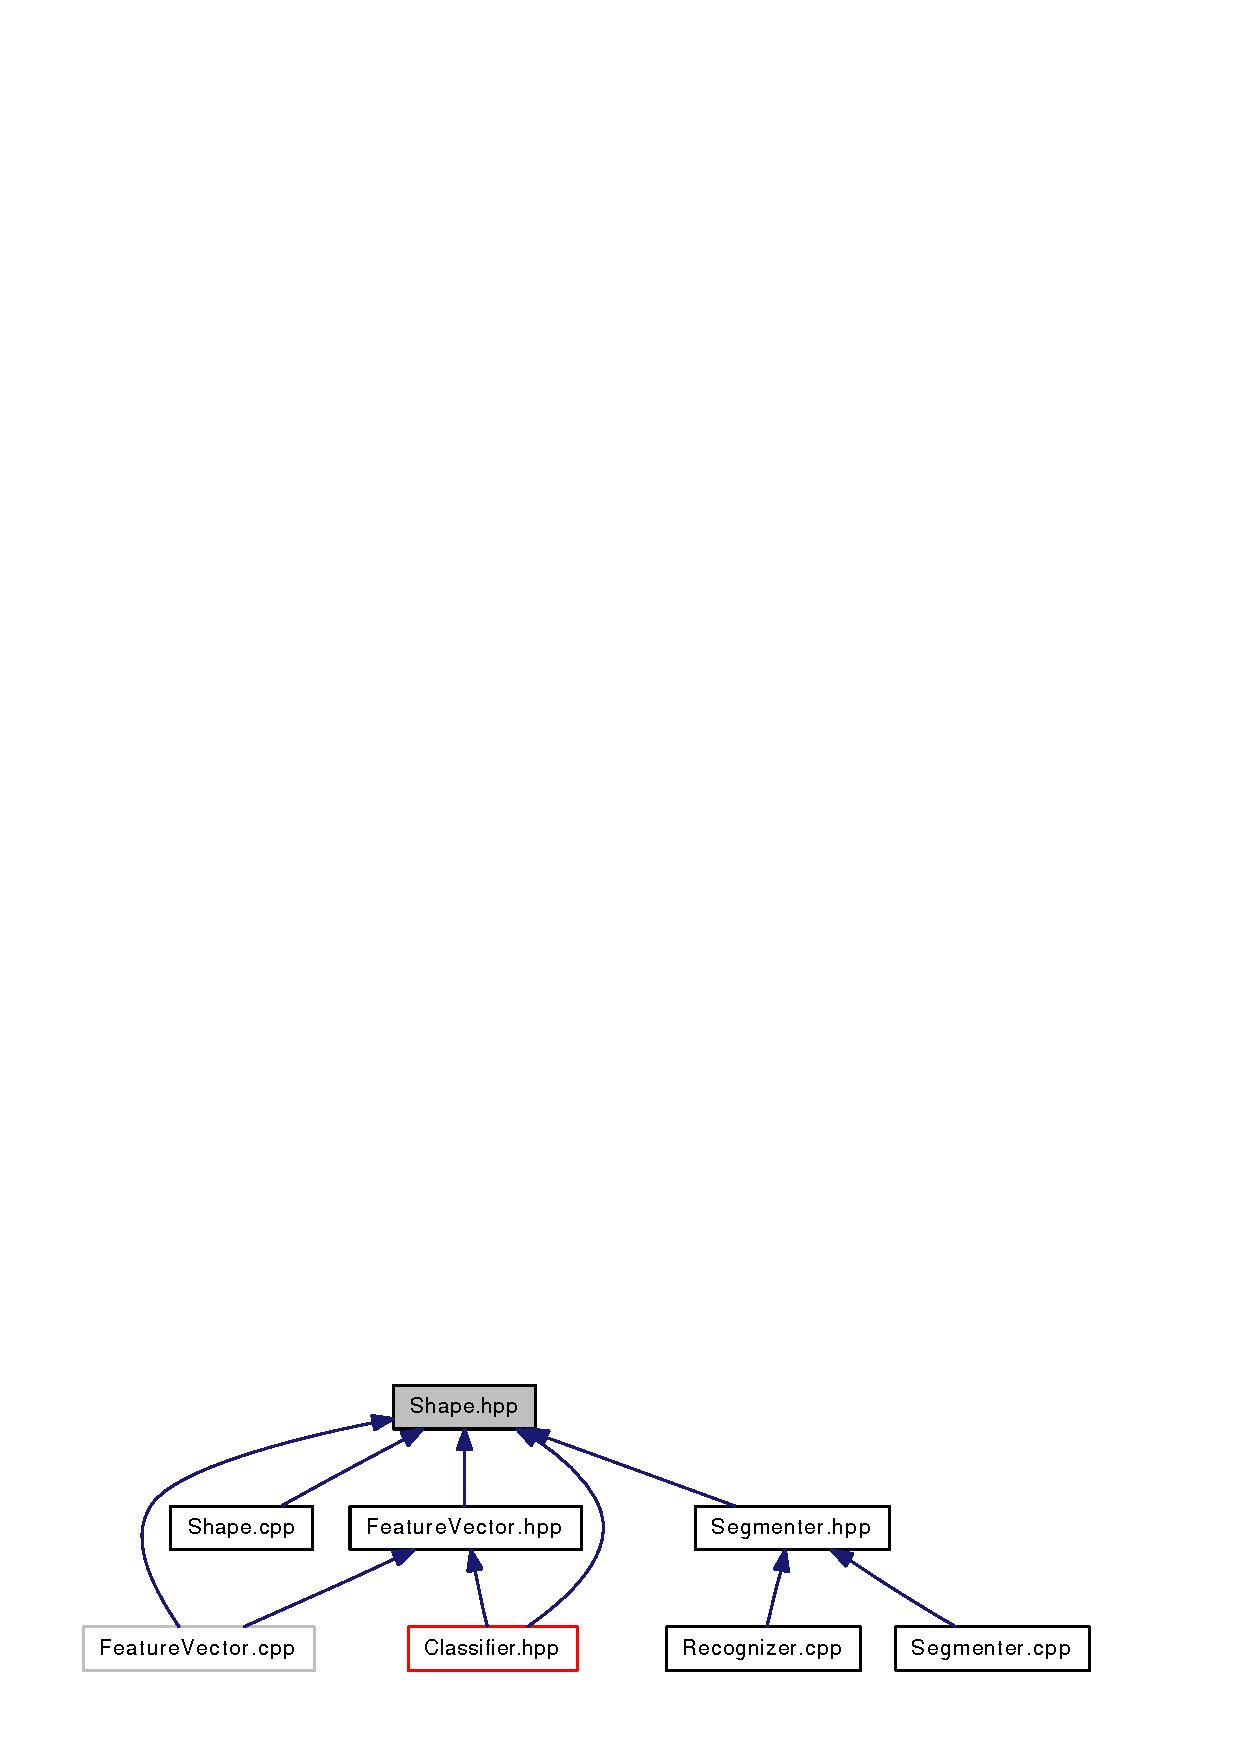
\includegraphics[width=187pt]{_shape_8hpp__dep__incl}
\end{center}
\end{figure}
\subsubsection*{Data Structures}
\begin{CompactItemize}
\item 
class \hyperlink{class_shape}{Shape}
\begin{CompactList}\small\item\em The shape of a character in a press clip. \item\end{CompactList}\end{CompactItemize}
\subsubsection*{Typedefs}
\begin{CompactItemize}
\item 
typedef std::pair$<$ unsigned int, unsigned int $>$ \hyperlink{_shape_8hpp_535e59456e3e633842529cfa8ea103c4}{Pixel}
\begin{CompactList}\small\item\em Coordinates of an image pixel. \item\end{CompactList}\end{CompactItemize}


\subsubsection{Detailed Description}
Declaration of \hyperlink{class_shape}{Shape} class. 



\subsubsection{Typedef Documentation}
\hypertarget{_shape_8hpp_535e59456e3e633842529cfa8ea103c4}{
\index{Shape.hpp@{Shape.hpp}!Pixel@{Pixel}}
\index{Pixel@{Pixel}!Shape.hpp@{Shape.hpp}}
\paragraph[{Pixel}]{\setlength{\rightskip}{0pt plus 5cm}{\bf Pixel}}\hfill}
\label{_shape_8hpp_535e59456e3e633842529cfa8ea103c4}


Coordinates of an image pixel. 

This pair keeps the coordinates of a pixel in a press clip. The first member representes the x coordinate (the row) and the second member representes the y coordinate (the column)

\begin{Desc}
\item[Author:]Eliezer Talón (\href{mailto:elitalon@gmail.com}{\tt elitalon@gmail.com}) \end{Desc}
\begin{Desc}
\item[Date:]2008-10-13 \end{Desc}
